\documentclass[10pt]{beamer}

\definecolor{dlightblue}{rgb}{0.65,0.65,0.98}
\definecolor{lightblue}{rgb}{0.85,0.85,1.0}
\definecolor{llightblue}{rgb}{0.95,0.95,0.98}
\definecolor{darkblue}{rgb}{0,0,.6}
\definecolor{darkred}{rgb}{.6,0,0}
\definecolor{darkgreen}{rgb}{0,.6,0}
\definecolor{darkbrown}{rgb}{0.5,0.30,0.10}
\definecolor{red}{rgb}{.98,0,0}

\definecolor{refcolor}{rgb}{0.0,0.6,0.0}
\setbeamercolor{upcol}{fg=black,bg=lightblue}
\setbeamercolor{lowcol}{fg=black,bg=llightblue}
\newenvironment{colorblock}
{\begin{beamerboxesrounded}[upper=upcol,lower=lowcol,shadow=false]}
{\end{beamerboxesrounded}}

\setbeamercolor{alertupcol}{fg=black,bg=dlightblue}
\setbeamercolor{alertlowcol}{fg=black,bg=lightblue}
\newenvironment{alertcolorblock}
{\begin{beamerboxesrounded}[upper=alertupcol,lower=alertlowcol,shadow=false]}
{\end{beamerboxesrounded}}
\setbeamercolor{block body}{bg=llightblue}
\setbeamercolor{block title}{fg=black,bg=lightblue}
\setbeamercovered{transparent}

\title[Quantum Annealing for Air Traffic Management]{Quantum Annealing for Air Traffic Management}
\author[Tobias Stollenwerk]
{\emph{Tobias Stollenwerk}\inst{1} \\
\vspace{0.3cm}
{\bf Collaborators\inst{2}} \\
Bryan O'Gorman,
Salvatore Mandr\`{a},
Davide Venturelli,
Eleanor G. Rieffel\\
{\bf Domain Experts}\inst{3} \\
Olga Rodionova,
Hok K. Ng,
Banavar Sridhar
}
\institute[NASA and DLR]
{\inst{1}
German Aerospace Center (DLR) \\
\inst{2}
NASA QuAIL \\
\inst{3}
NASA Aviation Systems Division
}
\date[QuAASI'16]{July 26, 2016}
\usetheme{dlr}
\begin{document}

\begin{frame}
    \titlepage
\end{frame}

\begin{frame}[t]{Content}
    \begin{itemize}
        \vspace{1.0cm}
        \item The problem of optimizing flight trajectories
        \vspace{0.3cm}
        \item Classical preprocessing
        \vspace{0.3cm}
        \item Mapping to Quadratic Unconstrained Binary Optimization (QUBO)
        \vspace{0.3cm}
        \item {\color{dlrgrey} Quantum annealing experiments (Work in progress)}
    \end{itemize}
\end{frame}

\begin{frame}[t]{Motivation}
	\begin{columns}[c]
        \hspace{0.1cm}
		\column{0.43\textwidth}
        \begin{block}{Today}
			\begin{center}
                    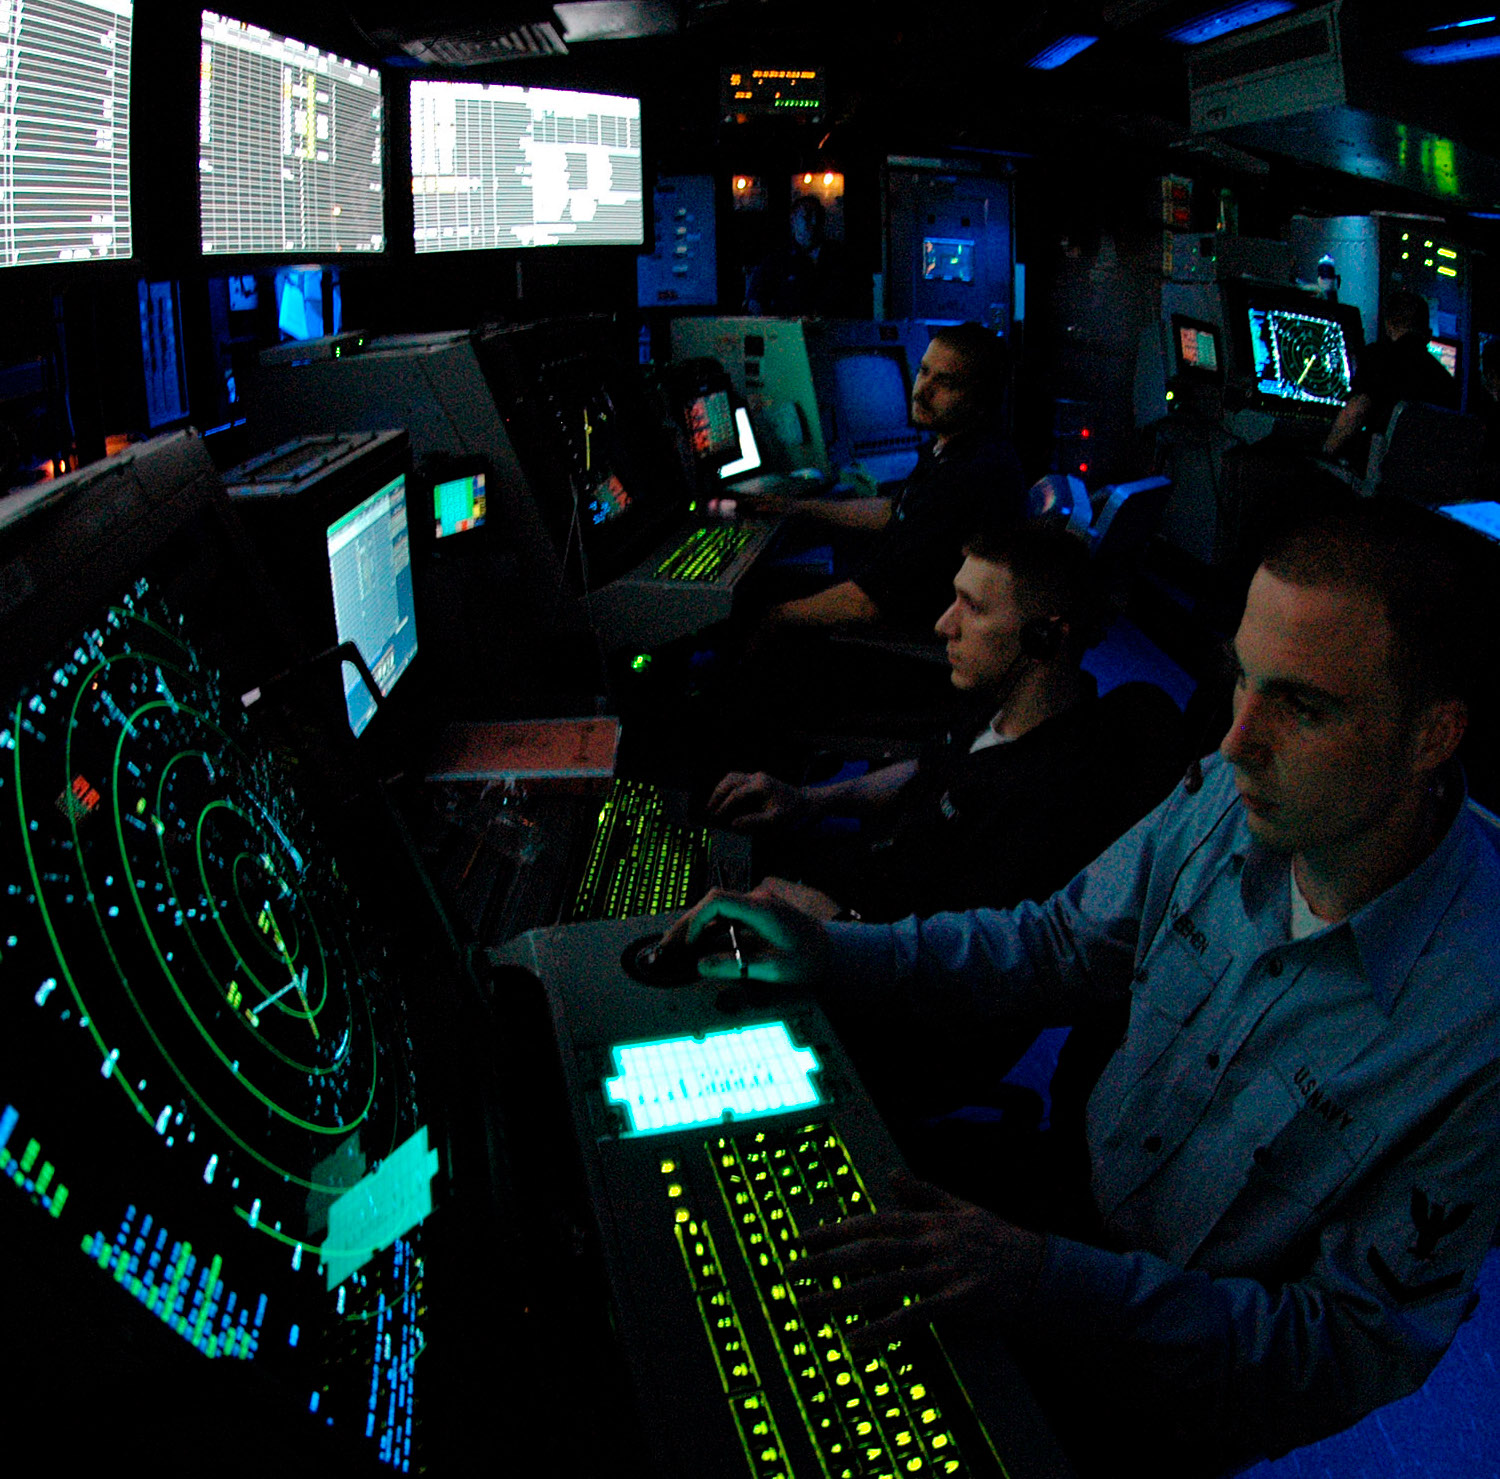
\includegraphics[width=0.6\textwidth]{images/atm_controller_small.jpg}
			\end{center}
            \begin{itemize}
                \item Manual conflict avoidance
                \item Computer support for humans
            \end{itemize}
        \end{block}
		\column{0.43\textwidth}
        \begin{block}{Future}
			\begin{center}
                    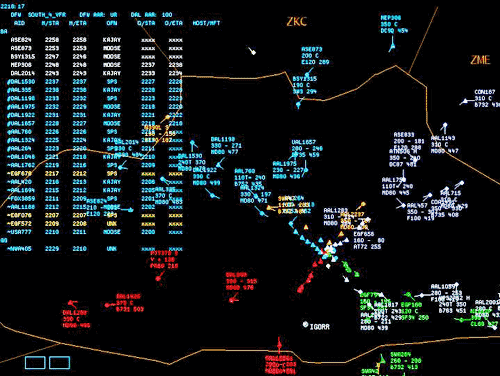
\includegraphics[width=0.65\textwidth]{images/atm_controller_software.png}
			\end{center}
            \begin{itemize}
                \item Increase in computer support for humans
                \item Precomputation of trajectories: Scheduling
            \end{itemize}
        \end{block}
	\end{columns}
\end{frame}
\begin{frame}[t]{Wind-Optimal Trajectories}
    \begin{itemize}
        \item 984 transatlantic flights on a single day
    \end{itemize}
    \begin{center}
        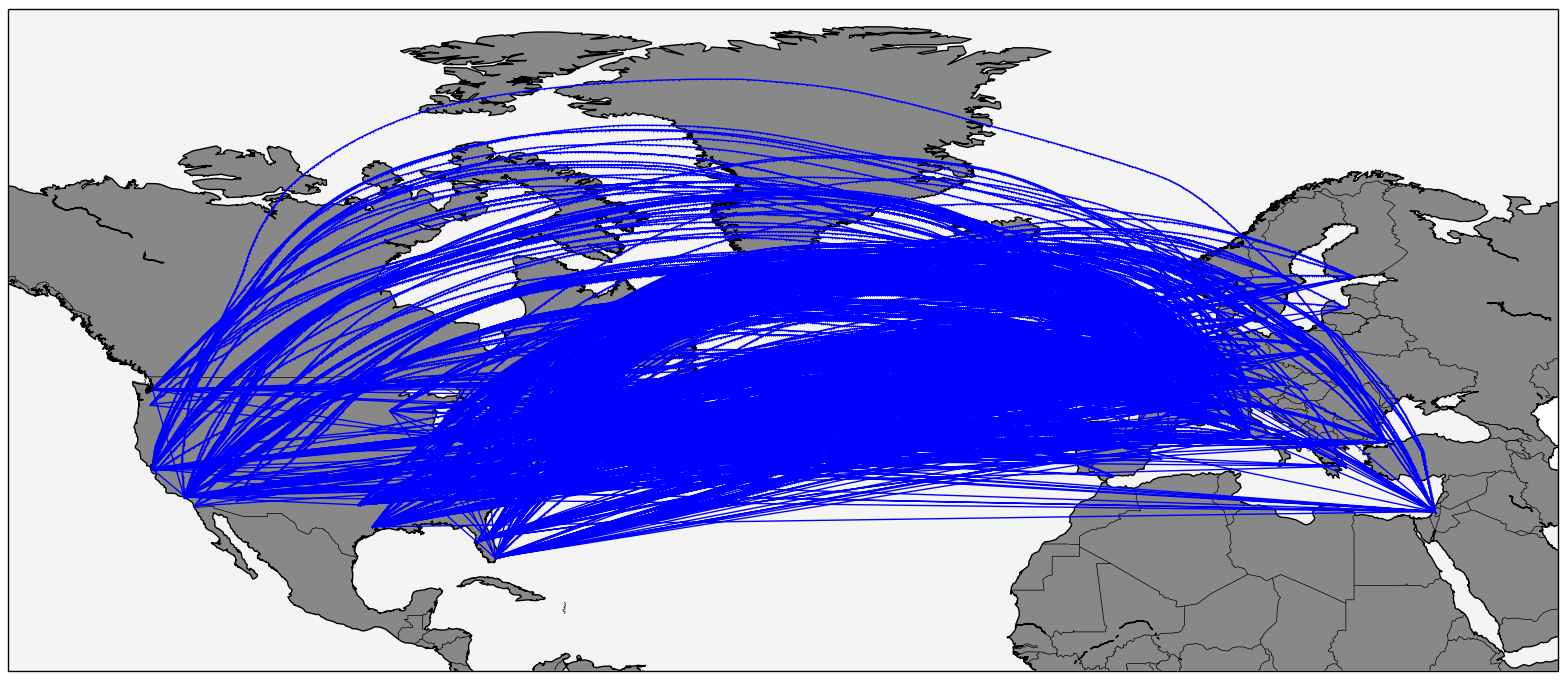
\includegraphics[width=1.0\textwidth]{images/wind_optimal_trajectories.png}
    \end{center}
    \vspace{-0.6cm}
    \hfill \tiny{Data from O. Rodionova}
\end{frame}
\begin{frame}[t]{Classical Optimization Based on Wind-Optimal Trajectories}
	\begin{columns}[c]
		\column{0.45\textwidth}
            \begin{itemize}
                \item Jetstream lead to narrow \emph{highways}
                \item Clusters of conflicting flights 
                \item Classical algorithm: Continuous deviation of trajectories
            \end{itemize}
            \begin{center}
                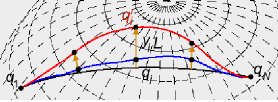
\includegraphics[width=1.0\textwidth]{images/classical_conflict_avoidance_half.png} \\
                \tiny{Rodionova et.\ al. (2016)}
            \end{center}
		\column{0.45\textwidth}
            \begin{center}
                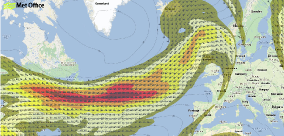
\includegraphics[width=1.0\textwidth]{images/classical_jetstream.png} \\
                \tiny{Woollings et.\ al. (2010)}
                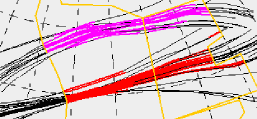
\includegraphics[width=1.0\textwidth]{images/classical_conflicts.png} \\
                \tiny{Rodionova et.\ al. (2016)}
            \end{center}
	\end{columns}
\end{frame}
\begin{frame}[t]{Optimization Problem Formulation}
    \begin{block}{Variables}
        \begin{itemize}
            \item Departure delays $d_i$ for each flight $i$
                \hspace{1cm}
                \begin{minipage}{0.3\linewidth}
                    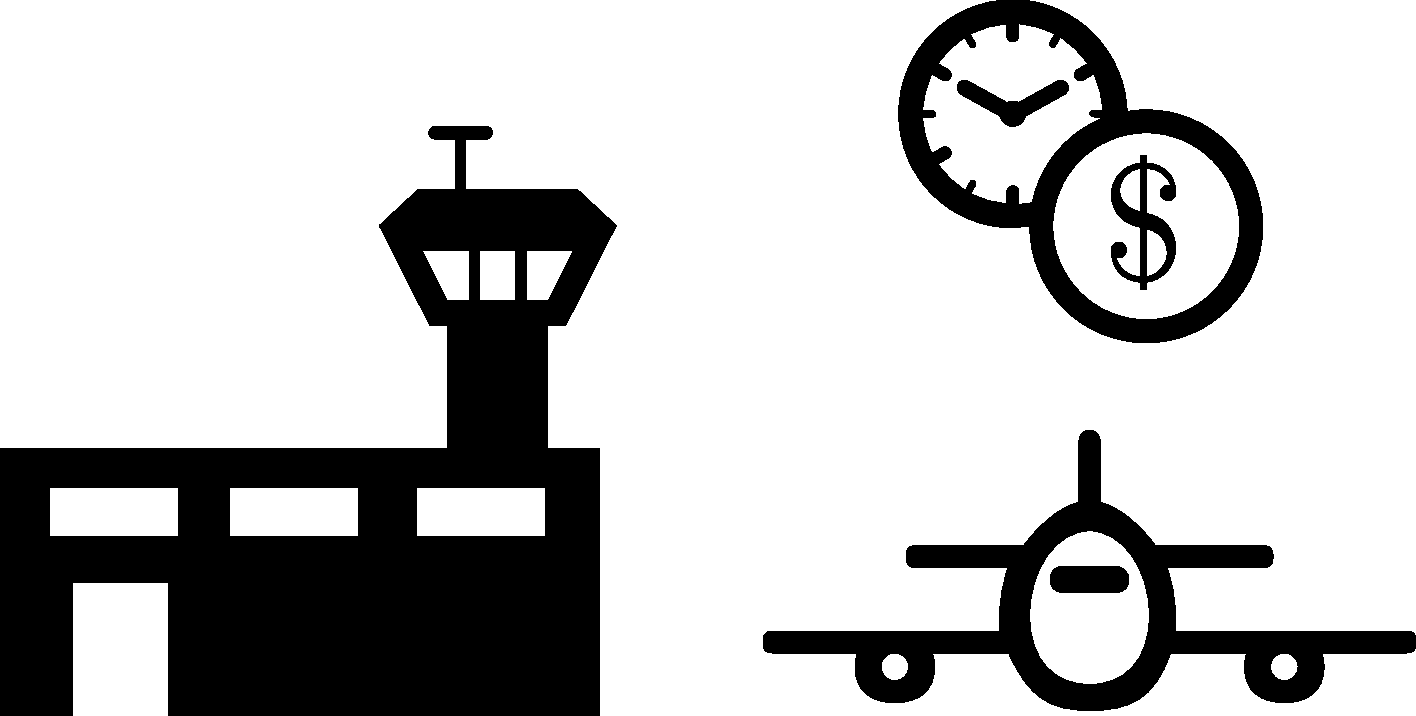
\includegraphics[width=0.8\textwidth]{images/departure_delay.pdf} \\
                \end{minipage}
            \item 
                \begin{minipage}[t]{0.5\linewidth}
                    Maneuver of flight $i$ to avoid conflict $k$ introduce delay $d_{ik}$
                \end{minipage}
                \hspace{1cm}
                \begin{minipage}[c]{0.3\linewidth}
                    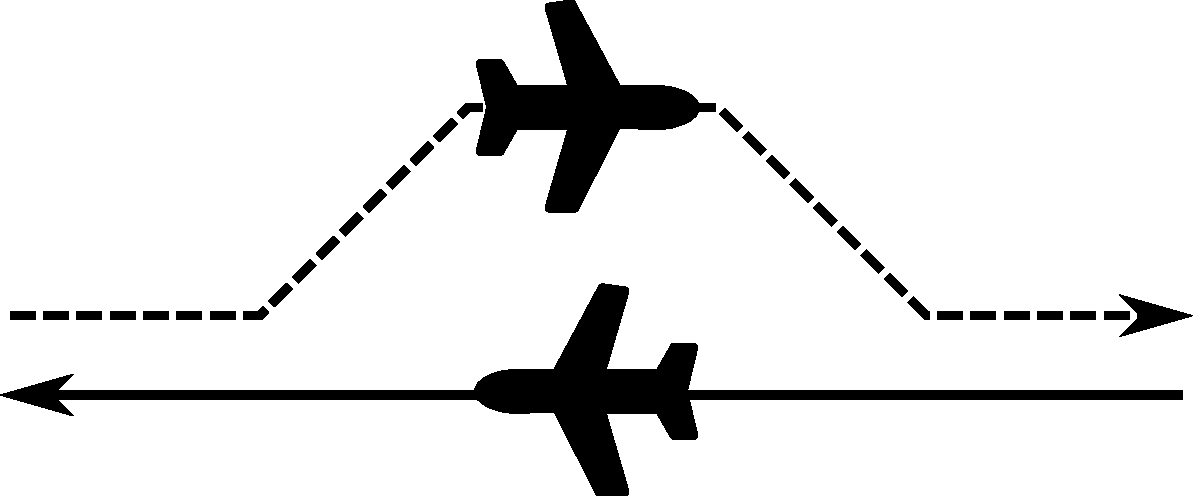
\includegraphics[width=0.9\textwidth]{images/conflict_avoiding_maneuver.pdf}
                \end{minipage}
       \end{itemize} 
    \end{block}
    \begin{block}{Cost function contribution}
        \centering
        Total delay: 
        $
            C = \sum_i d_i + \sum_{ik} d_{ik}
        $
    \end{block}
\end{frame}
 
\begin{frame}[t]{Optimization Problem Formulation - Simplifications}
    \begin{itemize}
        \item Only pairwise conflicts 
            \hfill
            \begin{minipage}[c]{0.6\linewidth}
                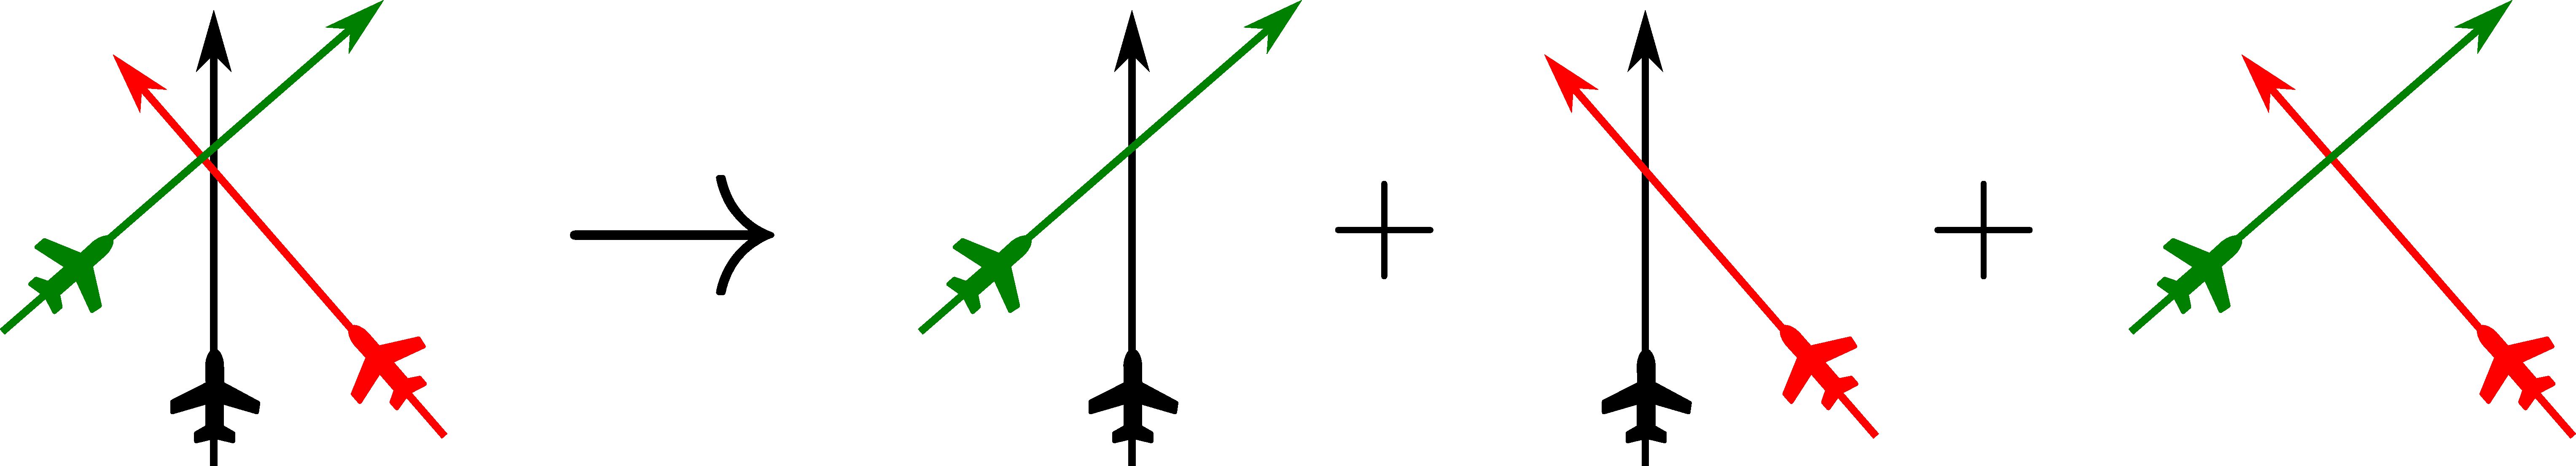
\includegraphics[width=0.9\textwidth]{images/pairwise_conflicts.pdf}
            \end{minipage}
            %\\
            %$\Rightarrow$ Each conflict $k$ is attached to exacly two flights $i_k$ $j_k$
        \item Conflict avoiding maneuvers impact {\bf only} on delay.
            \hfill
            \begin{minipage}[c]{0.3\linewidth}
                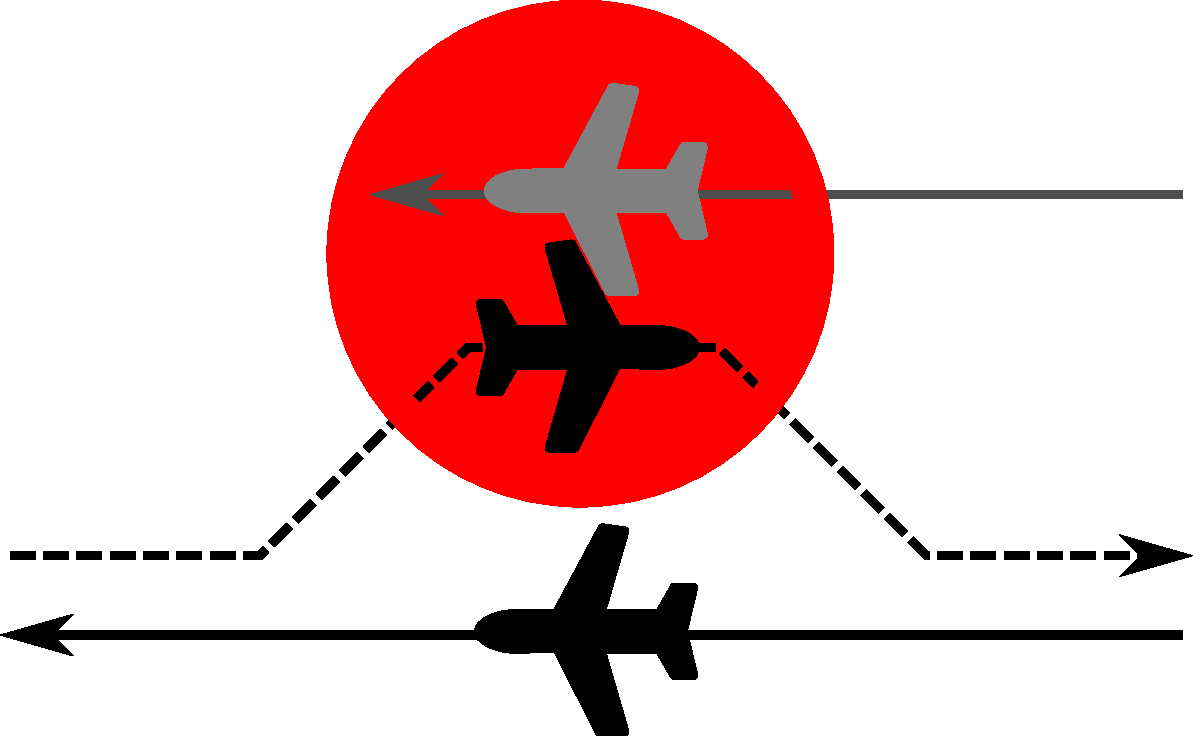
\includegraphics[width=0.9\textwidth]{images/conflict_avoiding_maneuver_pairwise_overlay1.pdf}
            \end{minipage}
    \end{itemize} 
\end{frame}
\begin{frame}[t]{Conflict Avoidance - Arrival Times}
    \begin{itemize}
        \item Difference of arrival times at the conflict between flights $i$ and $j$,  $\Delta_k = T_{ik} - T_{jk}$ \\
            \hspace{0.5cm}

            \begin{minipage}[c]{0.9\linewidth}
                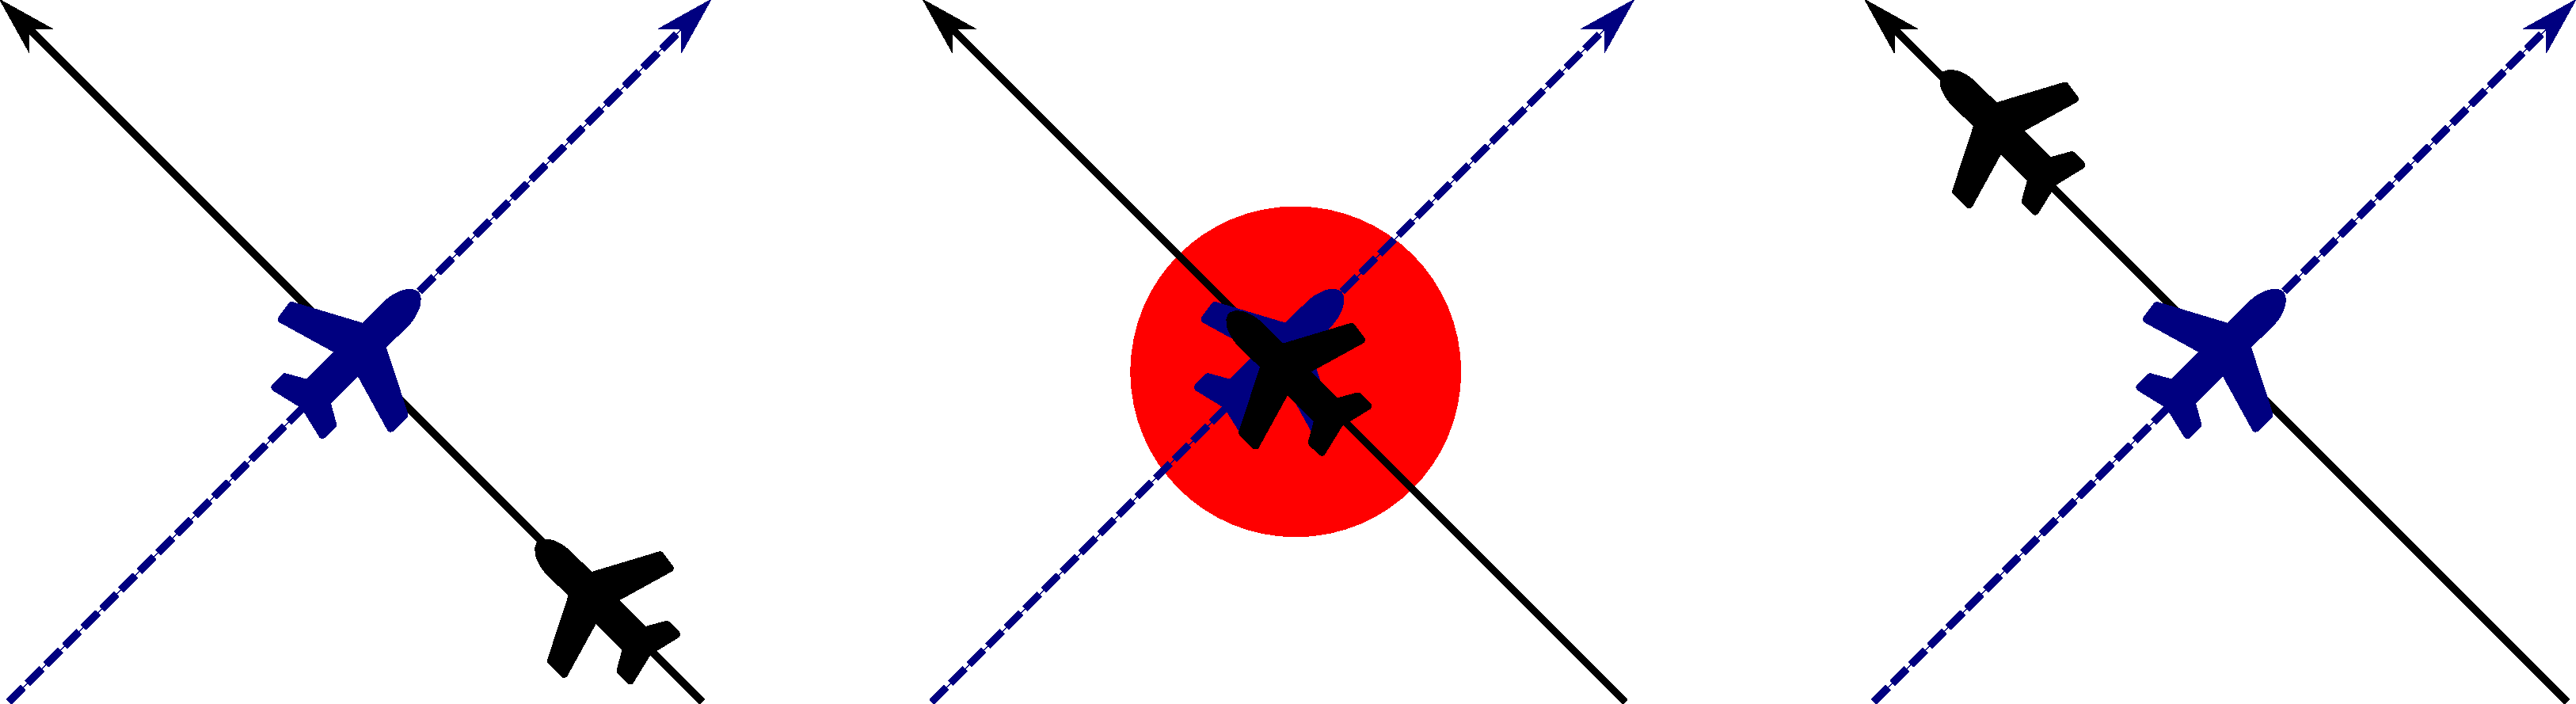
\includegraphics[width=1.0\textwidth]{images/conflict_avoiding_arrival_times.pdf}
                \\ 
            \end{minipage}
            \hspace{0.5cm}
            \\
            $\qquad \Delta_k \ll 0$
            $\qquad \qquad \qquad \Delta_k \approx 0$
            $\quad \qquad \qquad \qquad \Delta_k \gg 0$
        \item Delay resulting from conflict avoidance is function of $\Delta_k = T_{ik} - T_{jk}$:
            \begin{equation*}
                d_{ik} = \mathcal{D}_{ik}(\Delta_k)
            \end{equation*}
            \hfill 
            \begin{minipage}[c]{0.3\linewidth}
                \vspace{-1cm}
                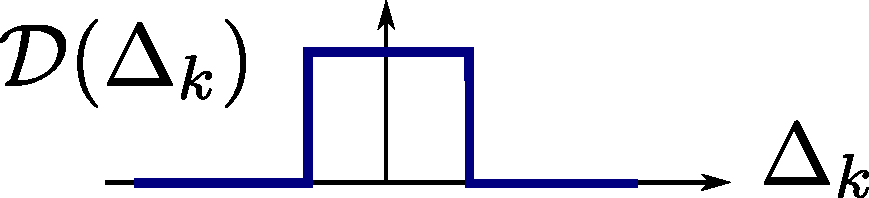
\includegraphics[width=1.0\textwidth]{images/conflict_delay_function.pdf}
            \end{minipage}
    \end{itemize} 
\end{frame}
\begin{frame}[t]{Conflict Avoidance - Maneuver Parameter}
    \begin{itemize}
        \item Maneuver parameter $a_k$, e.g. $a_k \in [0, 1]$
            \hfill
            \begin{minipage}[c]{0.9\linewidth}
                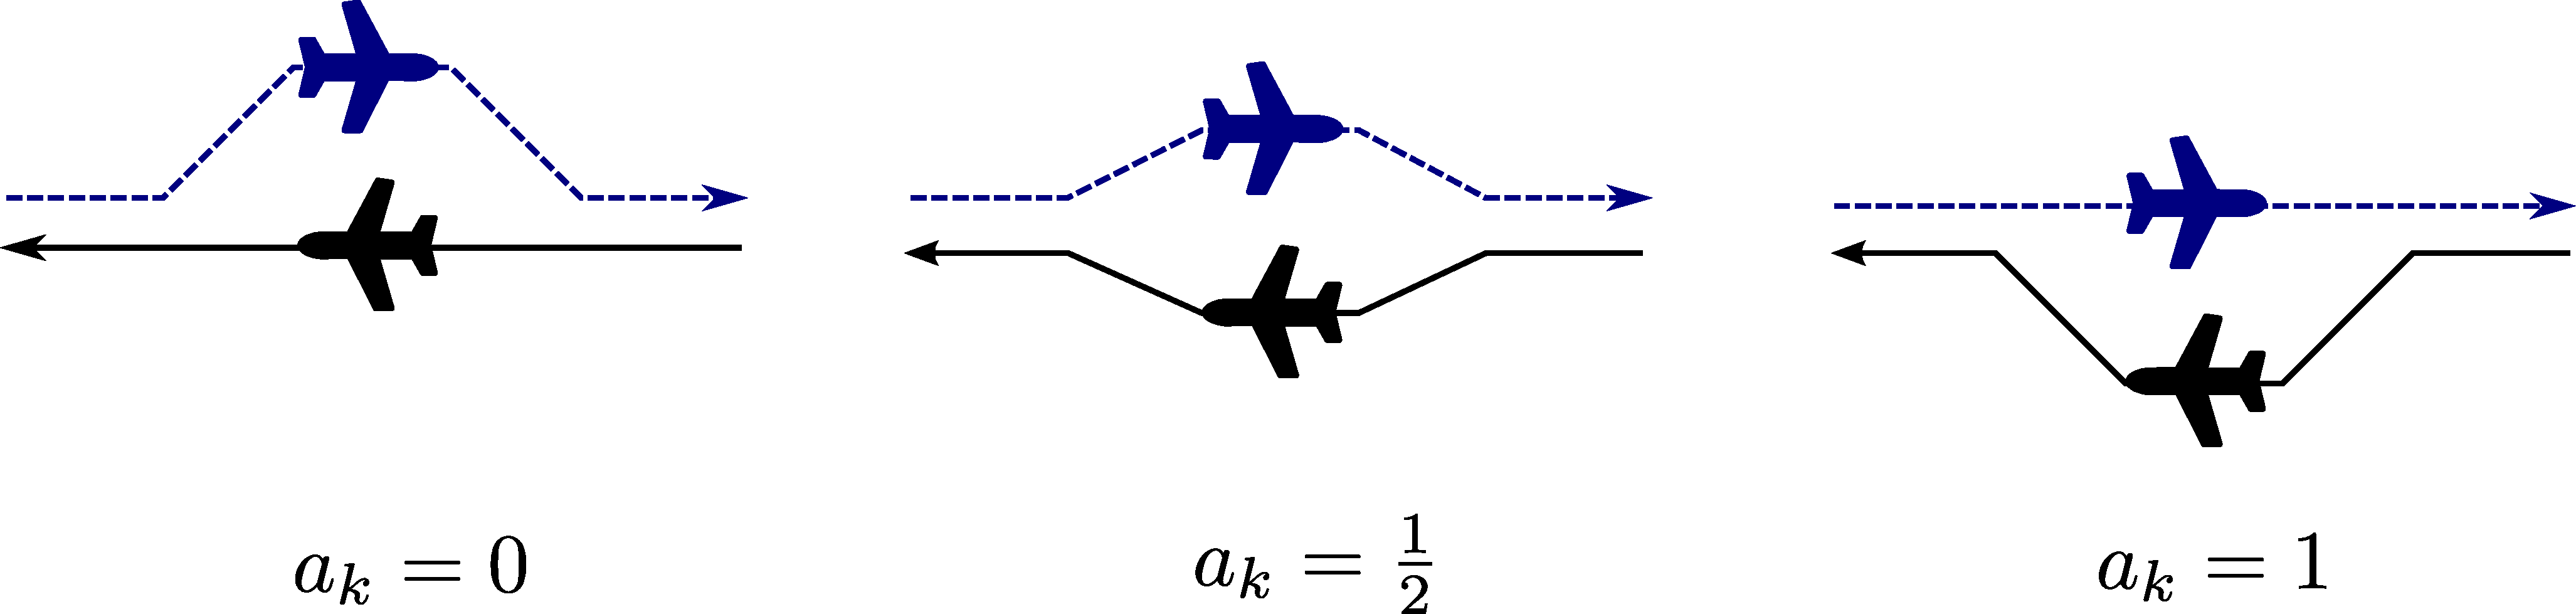
\includegraphics[width=1.0\textwidth]{images/conflict_avoiding_maneuver_parameter.pdf}
            \end{minipage}
        \item Delay resulting from conflict avoidance depends on maneuver:
            \begin{equation*}
                d_{ik} = \mathcal{D}_{ik}(\Delta_k, a_k) 
            \end{equation*}
    \end{itemize} 
    \begin{center}
    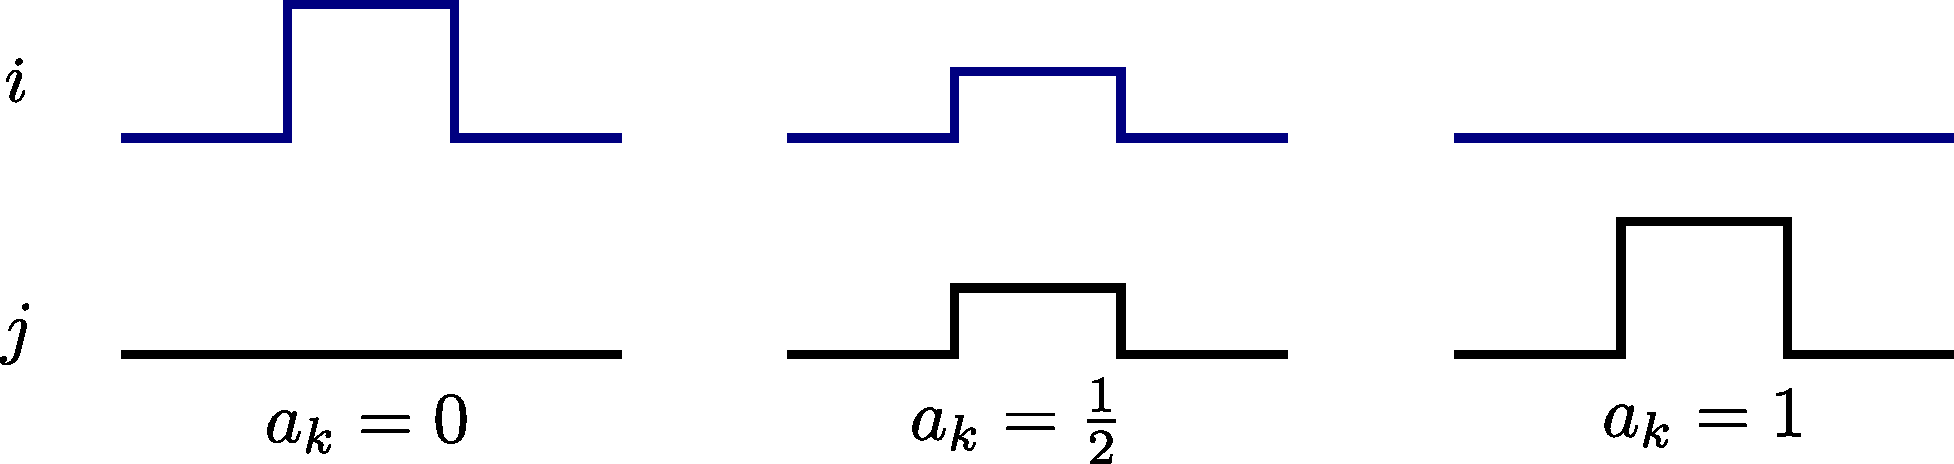
\includegraphics[width=0.76\textwidth]{images/conflict_delay_function_maneuver.pdf}
    \end{center}

\end{frame}


\begin{frame}[t]{Optimization Problem Formulation}
    \begin{itemize}
        \item Arrival time of flight $i$ at conflict $k$ is delayed by preceding conflicts
            \begin{equation*}
                T_{ik} = t_{ik} + d_i +  \sum_{p<k} d_{ip} \qquad t_{ik} \text{: Wind-optimal arrival time}
            \end{equation*}
        \item Optimization problem 
            \begin{equation*}
                \underset{d_i, d_{ik}, a_k}{\text{minimize}} \; \sum_i d_i + \sum_{ik} d_{ik}
            \end{equation*}
            \begin{align*}
                \text{subject to} \qquad
                & \Delta_{k} = t_{ik} + d_i + \sum_{p<k} d_{ip} - t_{jk} - d_j - \sum_{q<k} d_{jq} \\
                & d_{ik} = \mathcal{D}_{ik}(\Delta_{k}, a_k) 
            \end{align*}

    \end{itemize}
\end{frame}
\begin{frame}[t]{Precalculating Conflicts}
    \begin{minipage}[t]{0.4\linewidth}
        Given the trajectories of all flights $i$ 
    \end{minipage}
    \hfill
    \begin{minipage}[c]{0.5\linewidth}
        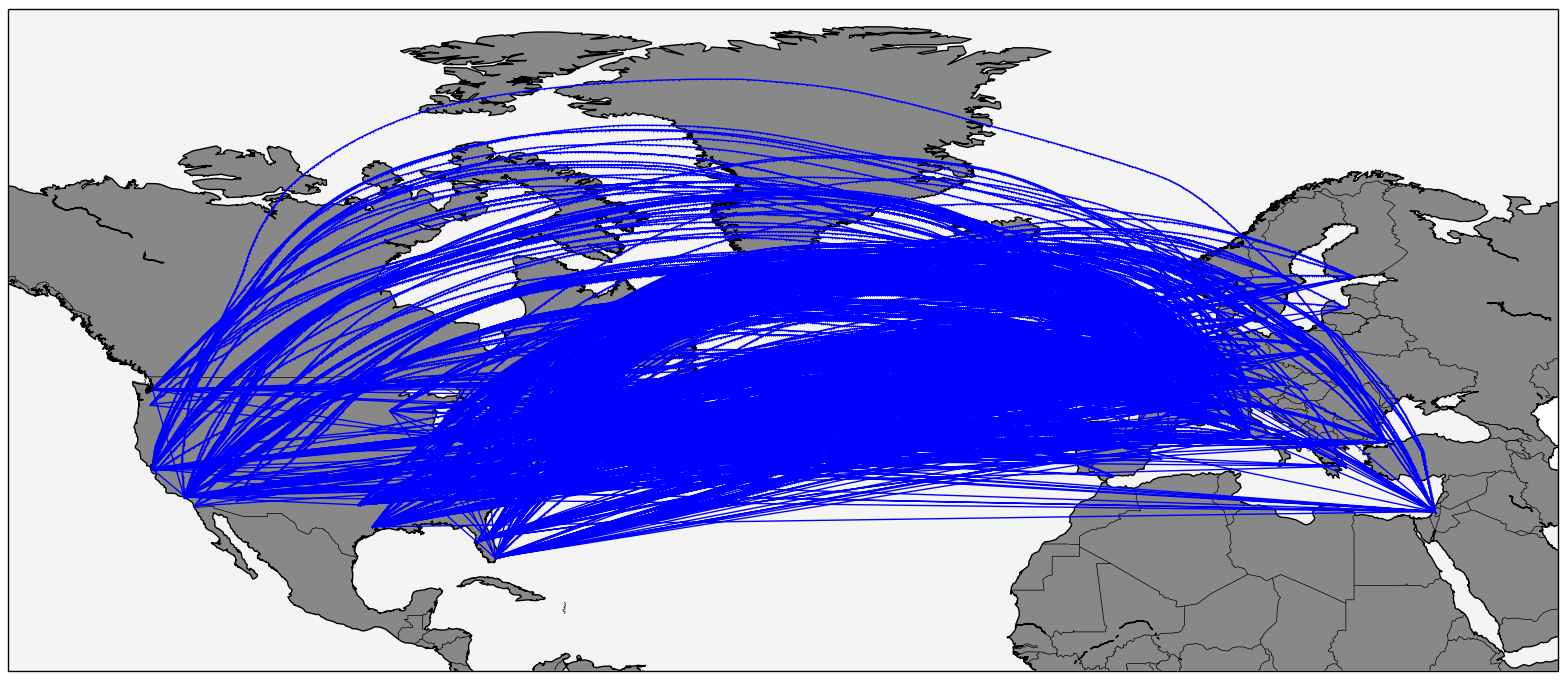
\includegraphics[width=1.0\textwidth]{images/wind_optimal_trajectories.png}
    \end{minipage}
    \vspace{1cm}
    \begin{center}
        $\Rightarrow$ How to calculate the \emph{potential} conflicts $k$?
    \end{center}
\end{frame}
%\begin{frame}[c]{}
    %\begin{center}
        %\hspace{-1cm}
        %{\LARGE Conflict Calculation}
    %\end{center}
%\end{frame}
\begin{frame}[t]{Spatial Conflict Detection}
    \begin{itemize}
        \item Spatial conflict, if trajectory points are close (3 nautical miles) to each other.
    \end{itemize}
    \begin{overprint}
	\begin{columns}[t]
        \visible<1-> {
		\column{0.45\textwidth}
            \begin{block}{Brute force algorithm}
                \begin{itemize}
                    \item Check distance between nearly {\bf all} trajectory points
                \end{itemize} 
                \begin{center}
                    \only<1>{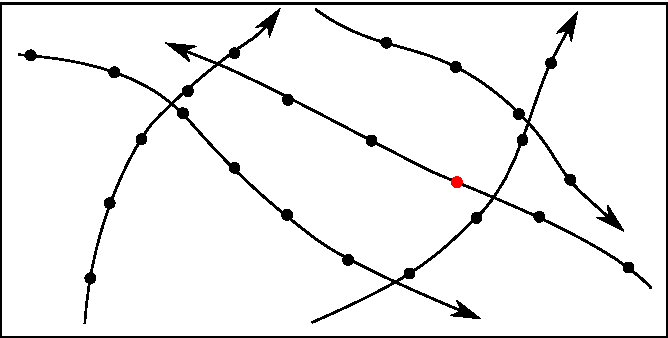
\includegraphics[width=1.0\textwidth]{images/spatial_conflict_detection_00.pdf}}
                    \only<2,3,4>{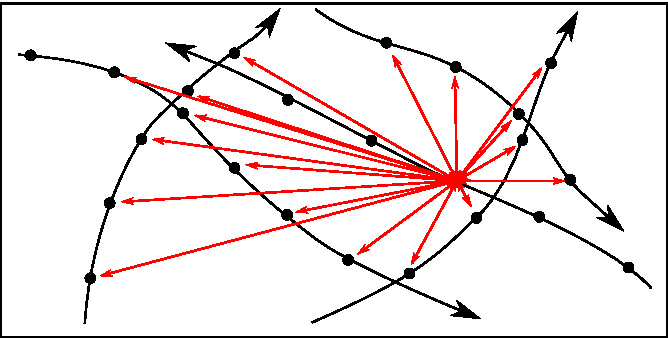
\includegraphics[width=1.0\textwidth]{images/spatial_conflict_detection_01.pdf}}
                \end{center}
            \end{block}
        }
        \visible<3-> {
		\column{0.45\textwidth}
            \begin{block}{Coarse grid algorithm}
                \begin{itemize}
                    \item Map trajectory points to coarse grid
                \end{itemize} 
                \begin{center}
                    \only<3>{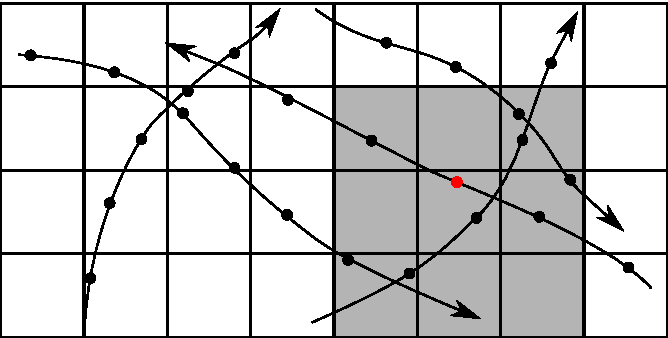
\includegraphics[width=1.0\textwidth]{images/spatial_conflict_detection_02.pdf}}
                    \only<4>{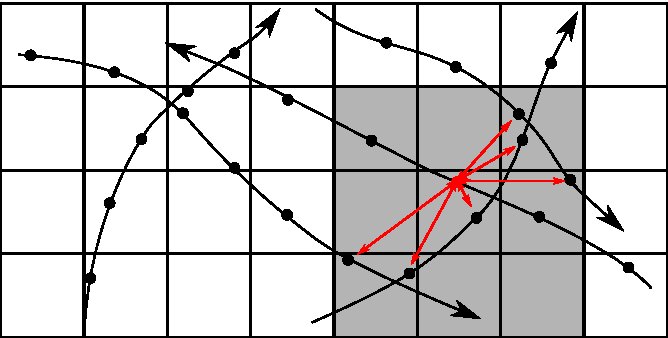
\includegraphics[width=1.0\textwidth]{images/spatial_conflict_detection_03.pdf}}
                \end{center}
                \visible<4> {
                \vspace{-0.3cm}
                \begin{itemize}
                    \item Check distance only with neighboring cells
                \end{itemize} 
                }
            \end{block}
        }
    \end{columns}
        
    \end{overprint}
\end{frame}
\begin{frame}[t]{Potential Conflicts}
    \begin{itemize}
        \item Potential conflict: Spatial conflict which can become real conflict
            \hspace{0.5cm}

            \begin{minipage}[c]{0.9\linewidth}
                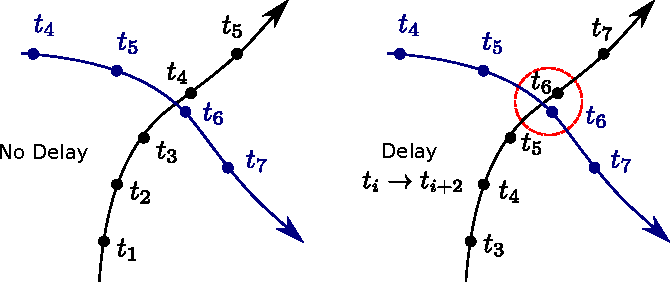
\includegraphics[width=1.0\textwidth]{images/potential_conflict.pdf}
                \\ 
            \end{minipage}
            \\
            \hspace{1.0cm}
            Spatial Conflict
            \hspace{3cm}
            Real Conflict
        \item First step: Potential conflict, if difference in wind-optimal arrival times $t_{ik}-t_{jk} < 2 $ hours.
    \end{itemize} 
\end{frame}

\begin{frame}[t]{Potential Conflicts}
    \begin{itemize}
        \item How to reduce the huge number of potential conflicts: $N_\text{conflict} = 43251$?
    \end{itemize}
    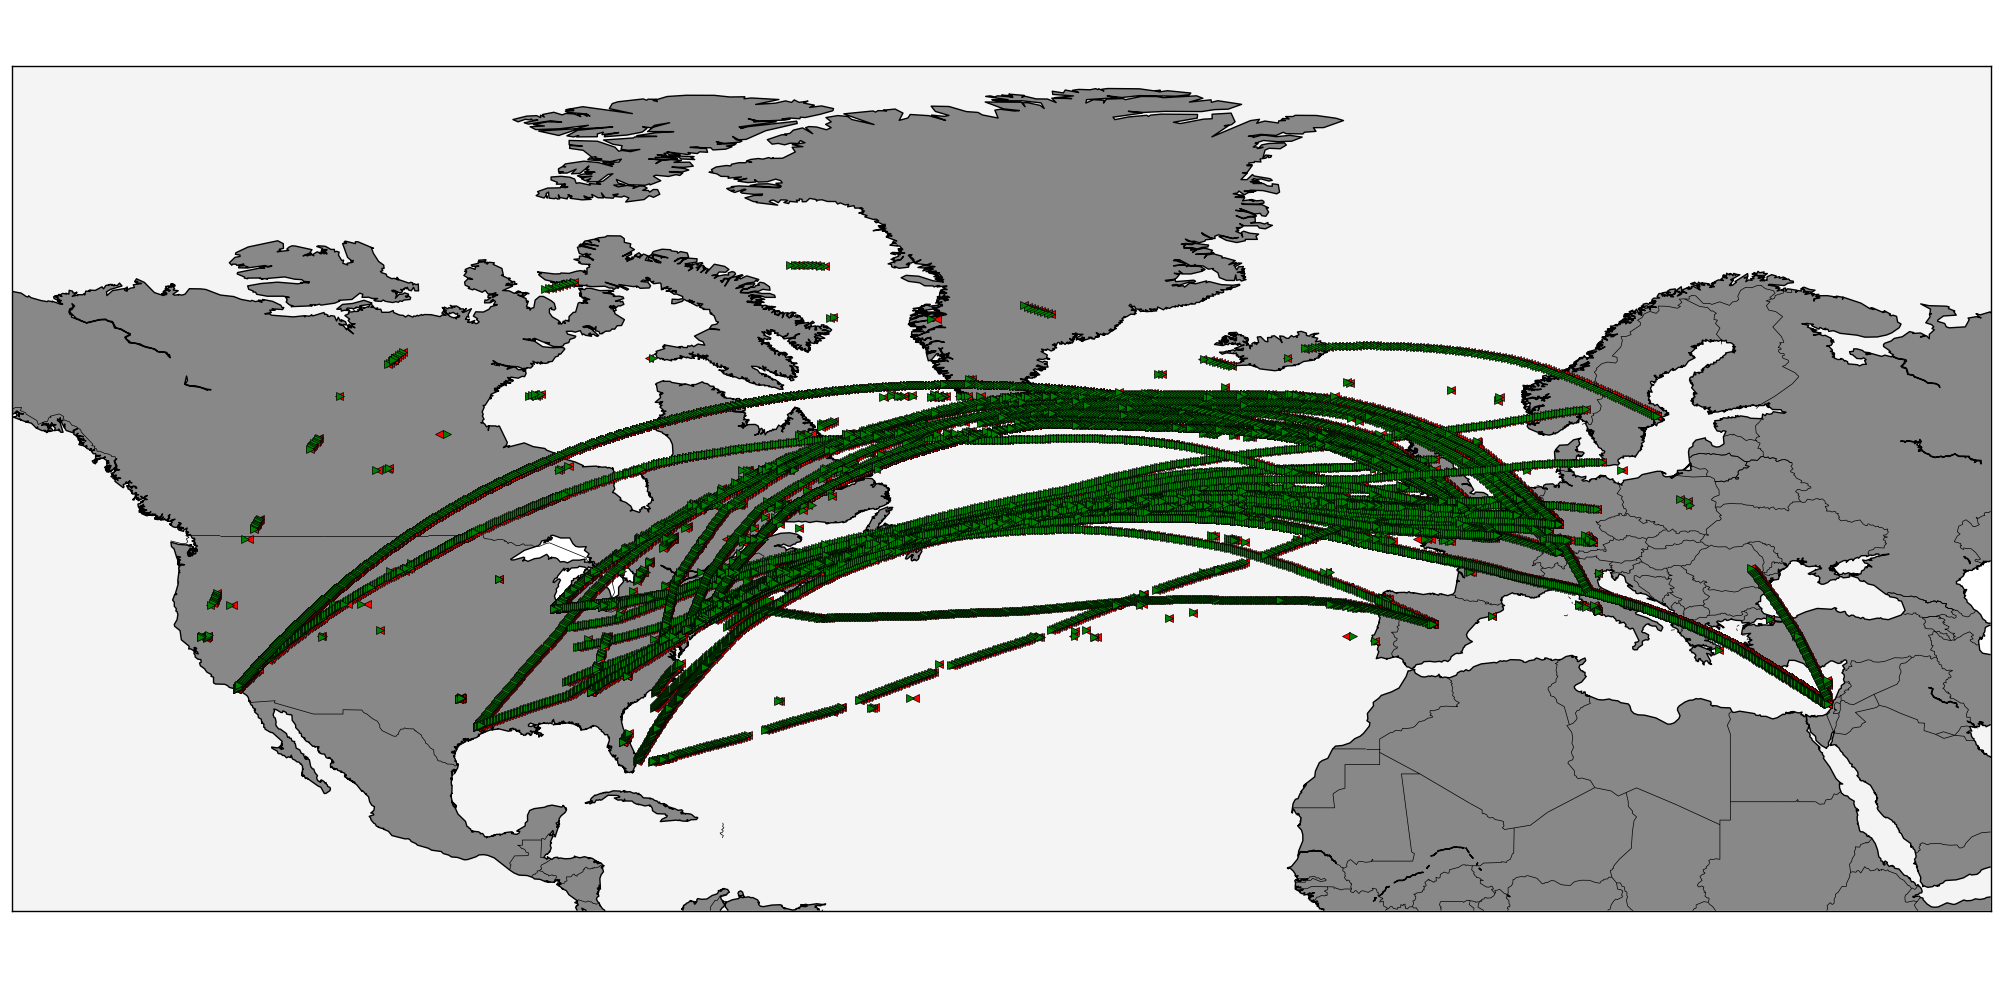
\includegraphics[width=1.0\textwidth]{images/spatial_conflicts_data.png}
\end{frame}
\begin{frame}[t]{Potential Conflicts - Classification}
    Reduce the vast number of potential conflicts by categorizing:
    \begin{itemize}
        \item Point Conflict: Isolated in time $N_\text{point} = 3573$
        \item Parallel conflict: Point conflicts consecutive in time $N_\text{parallel} = 2510$
        \item Reduction of $86 \%$
    \end{itemize}
    \begin{center}
        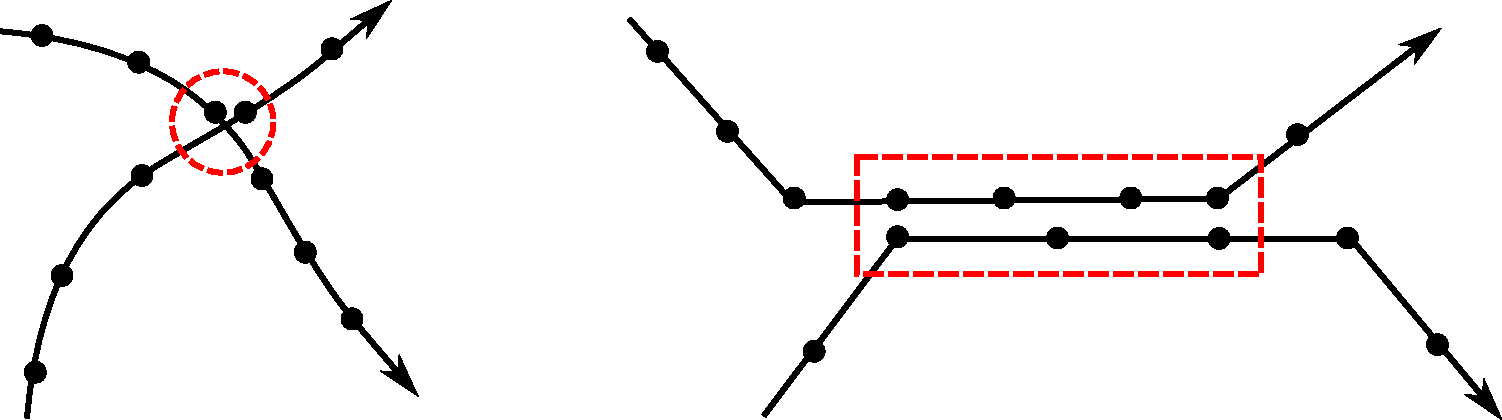
\includegraphics[width=0.9\textwidth]{images/spatial_conflict_categories.pdf}
    \end{center}
    \hspace{1.0cm}
    Point Conflict
    \hspace{3.5cm}
    Parallel Conflict
\end{frame}
\begin{frame}[t]{Potential Conflicts - Reduction}
    Self-consistent algorithm:
    \begin{itemize}
        \item For each flight, order conflicts in time
        \item For each potential conflict, calculate the maximal delay of both flights
        \item Remove potential conflicts which can not become real conflicts
        \item Repeat the above steps until convergence ($N_\text{conflict}$ invariant) 
    \end{itemize}
    \begin{center}
        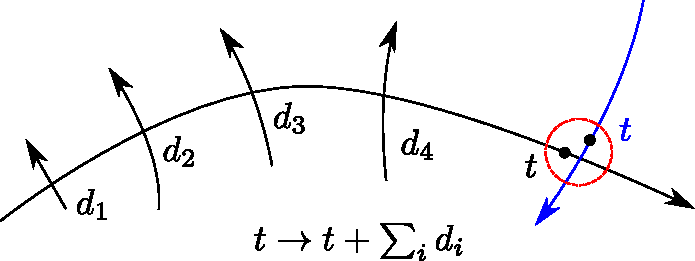
\includegraphics[width=0.8\textwidth]{images/potential_conflict_detection.pdf}
    \end{center}
\end{frame}
\begin{frame}[t]{Potential Conflicts - Reduction}
    \begin{center}
        \hspace{-1.5cm}
        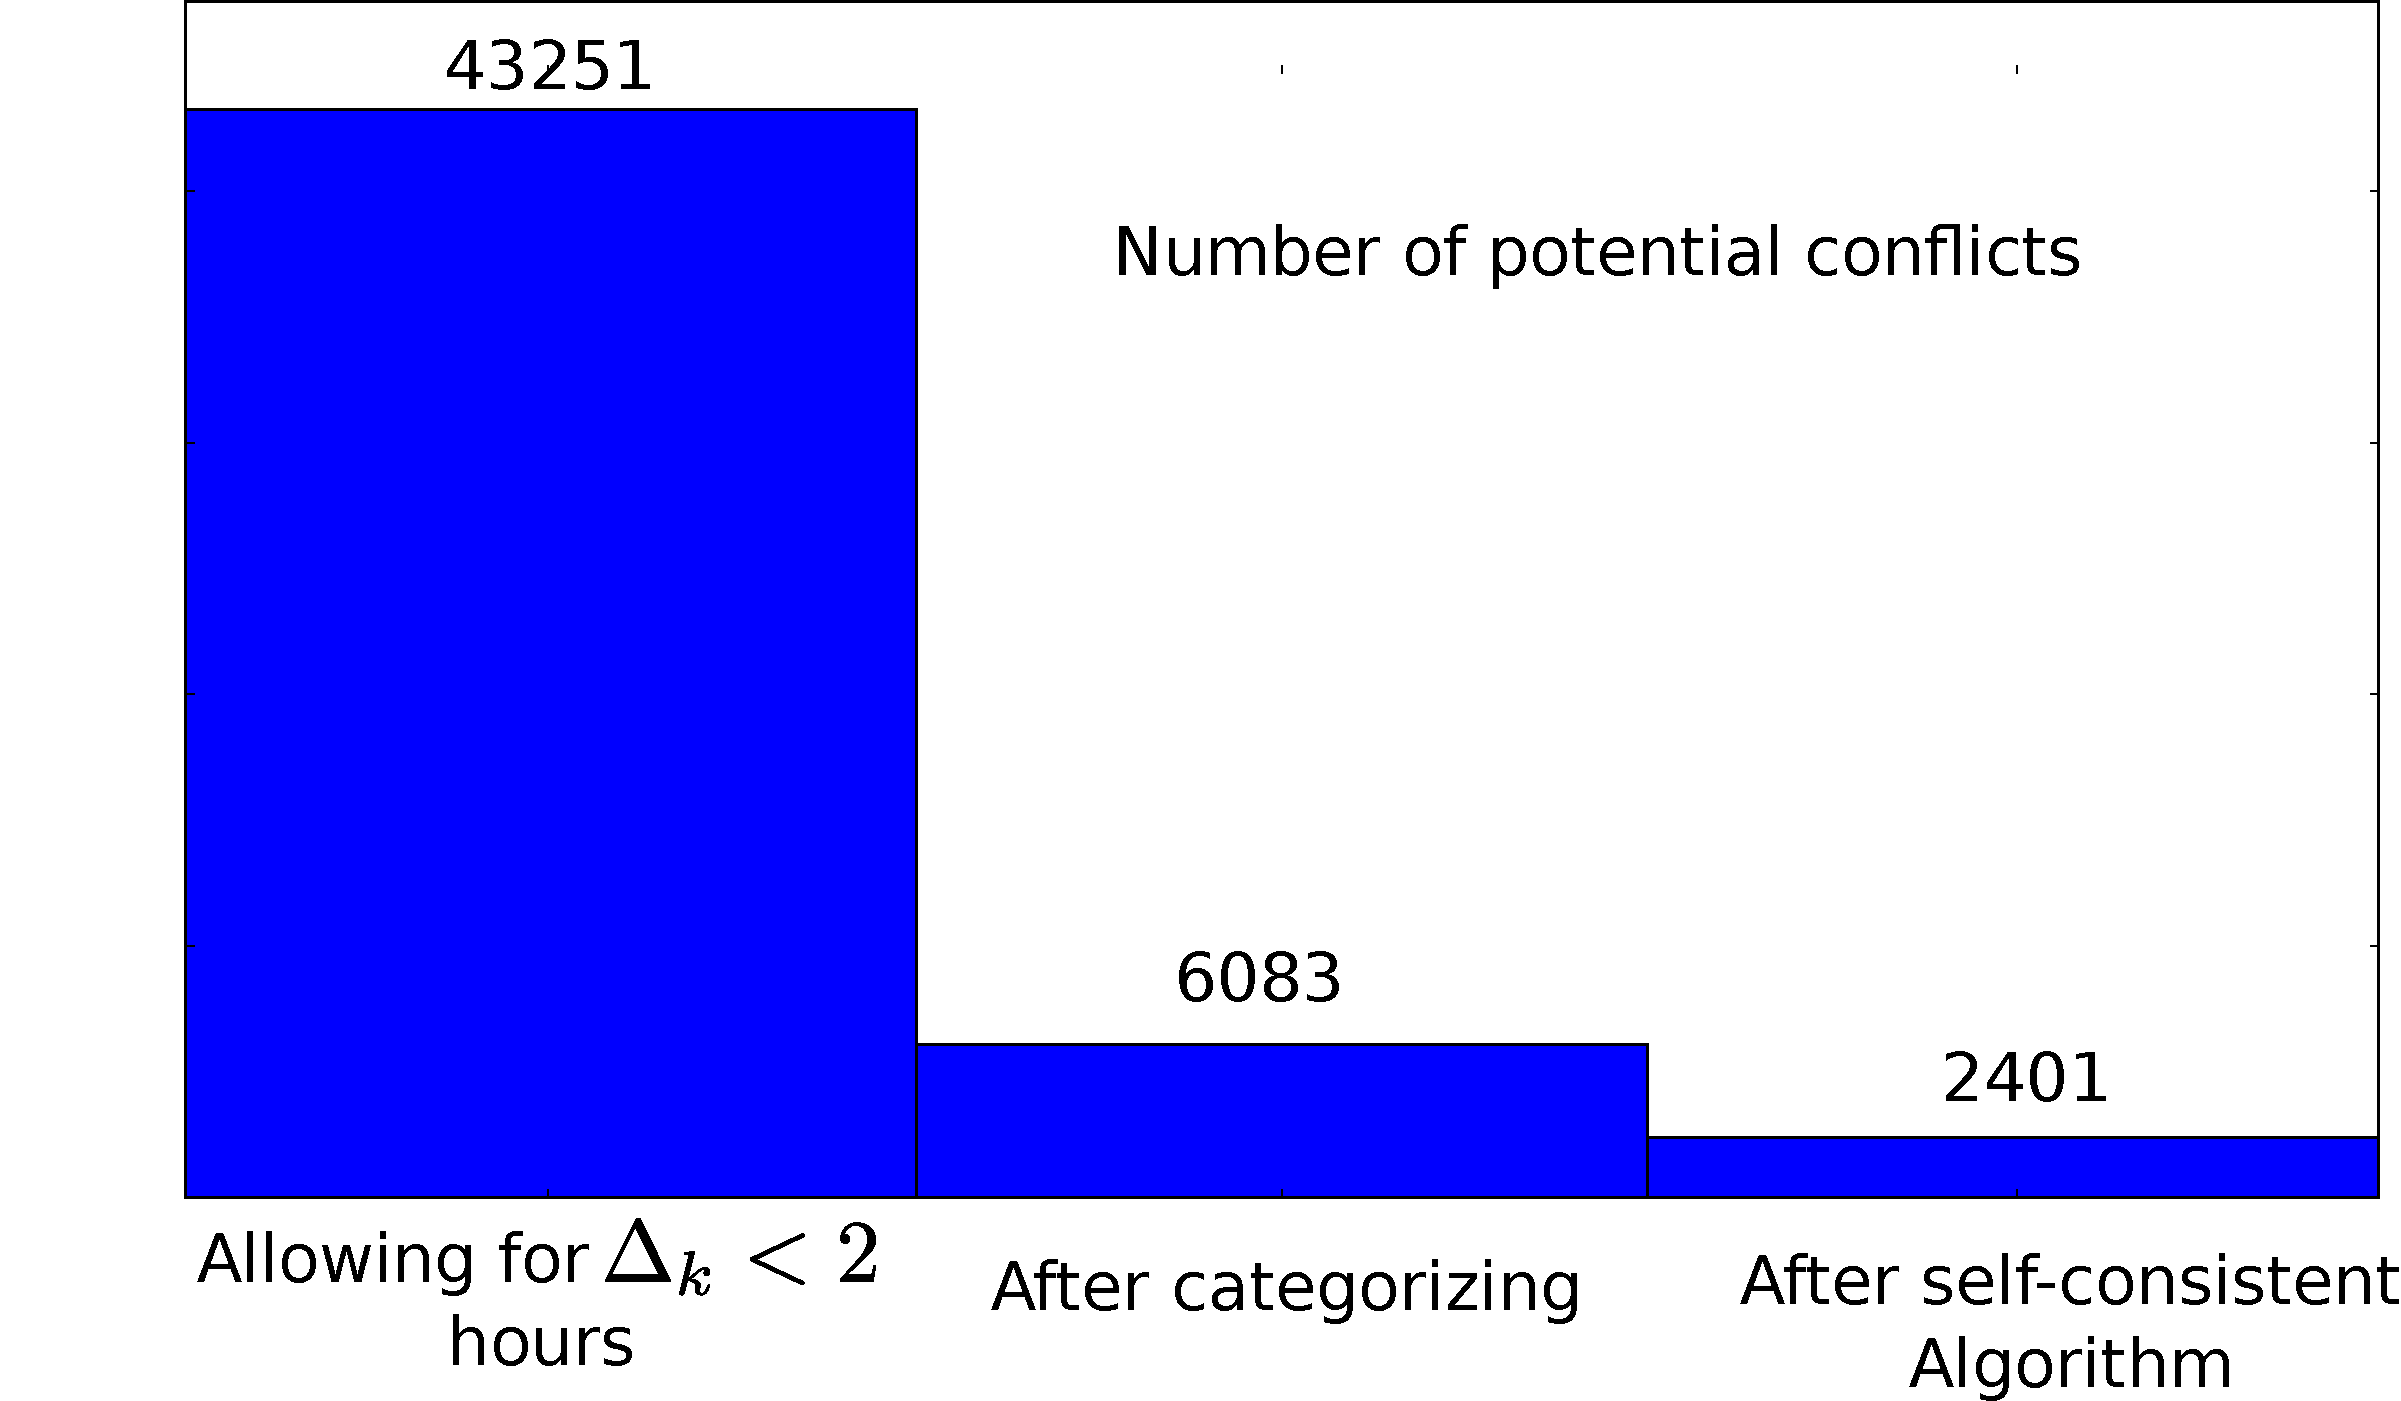
\includegraphics[width=0.8\textwidth]{images/potential_conflict_reduction.pdf}
    \end{center}
\end{frame}
\begin{frame}[t]{Potential Conflicts - Disconnected Subsets}
    \only<1> {
        \begin{center}
            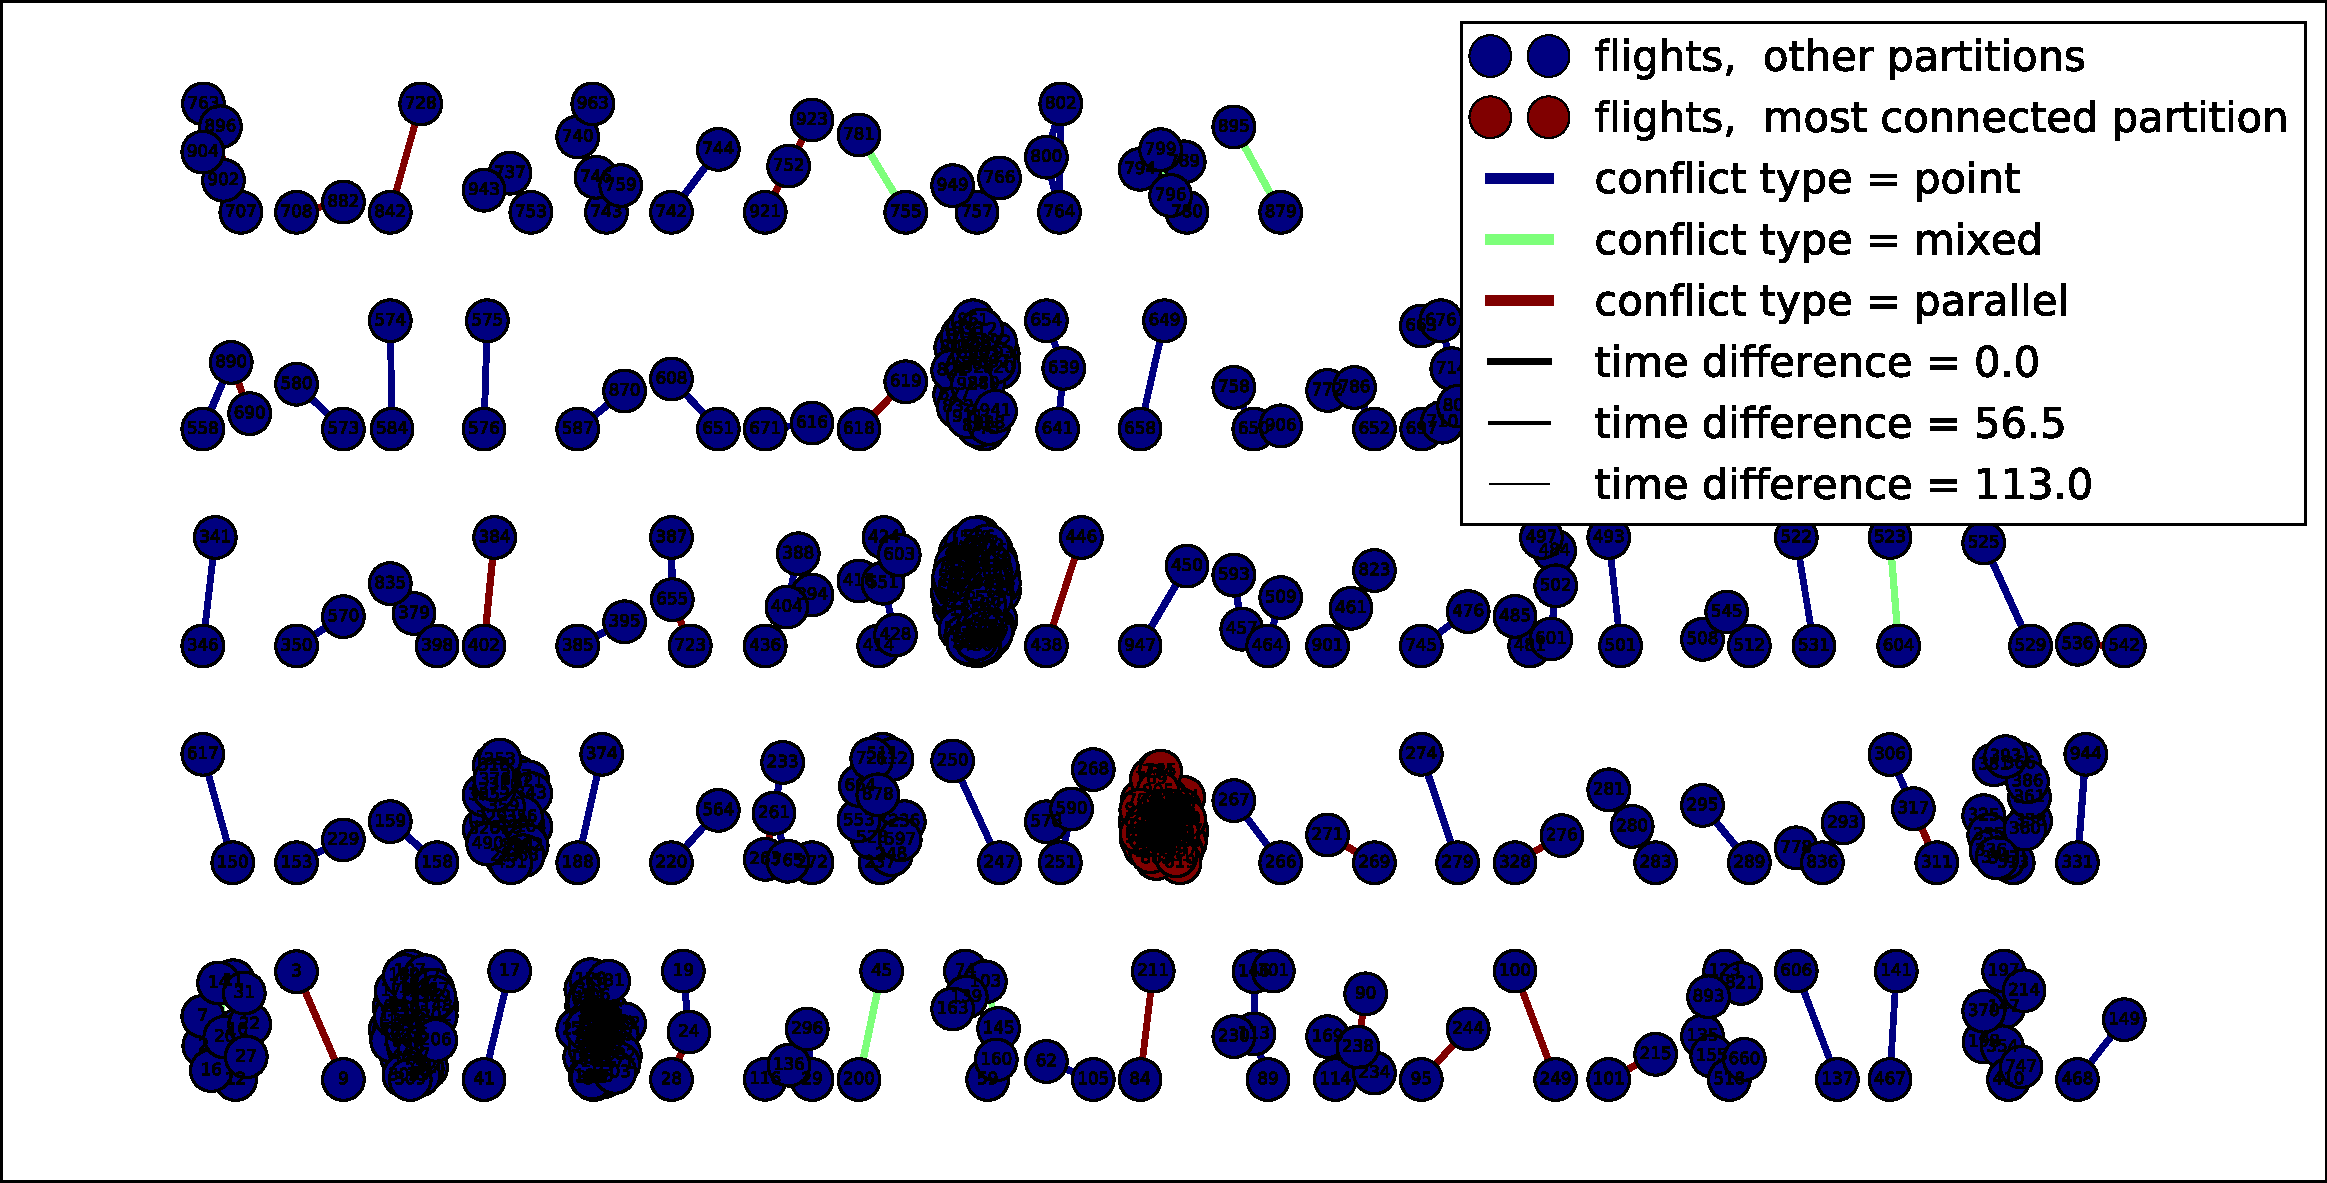
\includegraphics[width=0.85\textwidth]{images/conflicts_graph_new.pdf}
        \end{center}
    }
    \only<2> {
        \begin{center}
            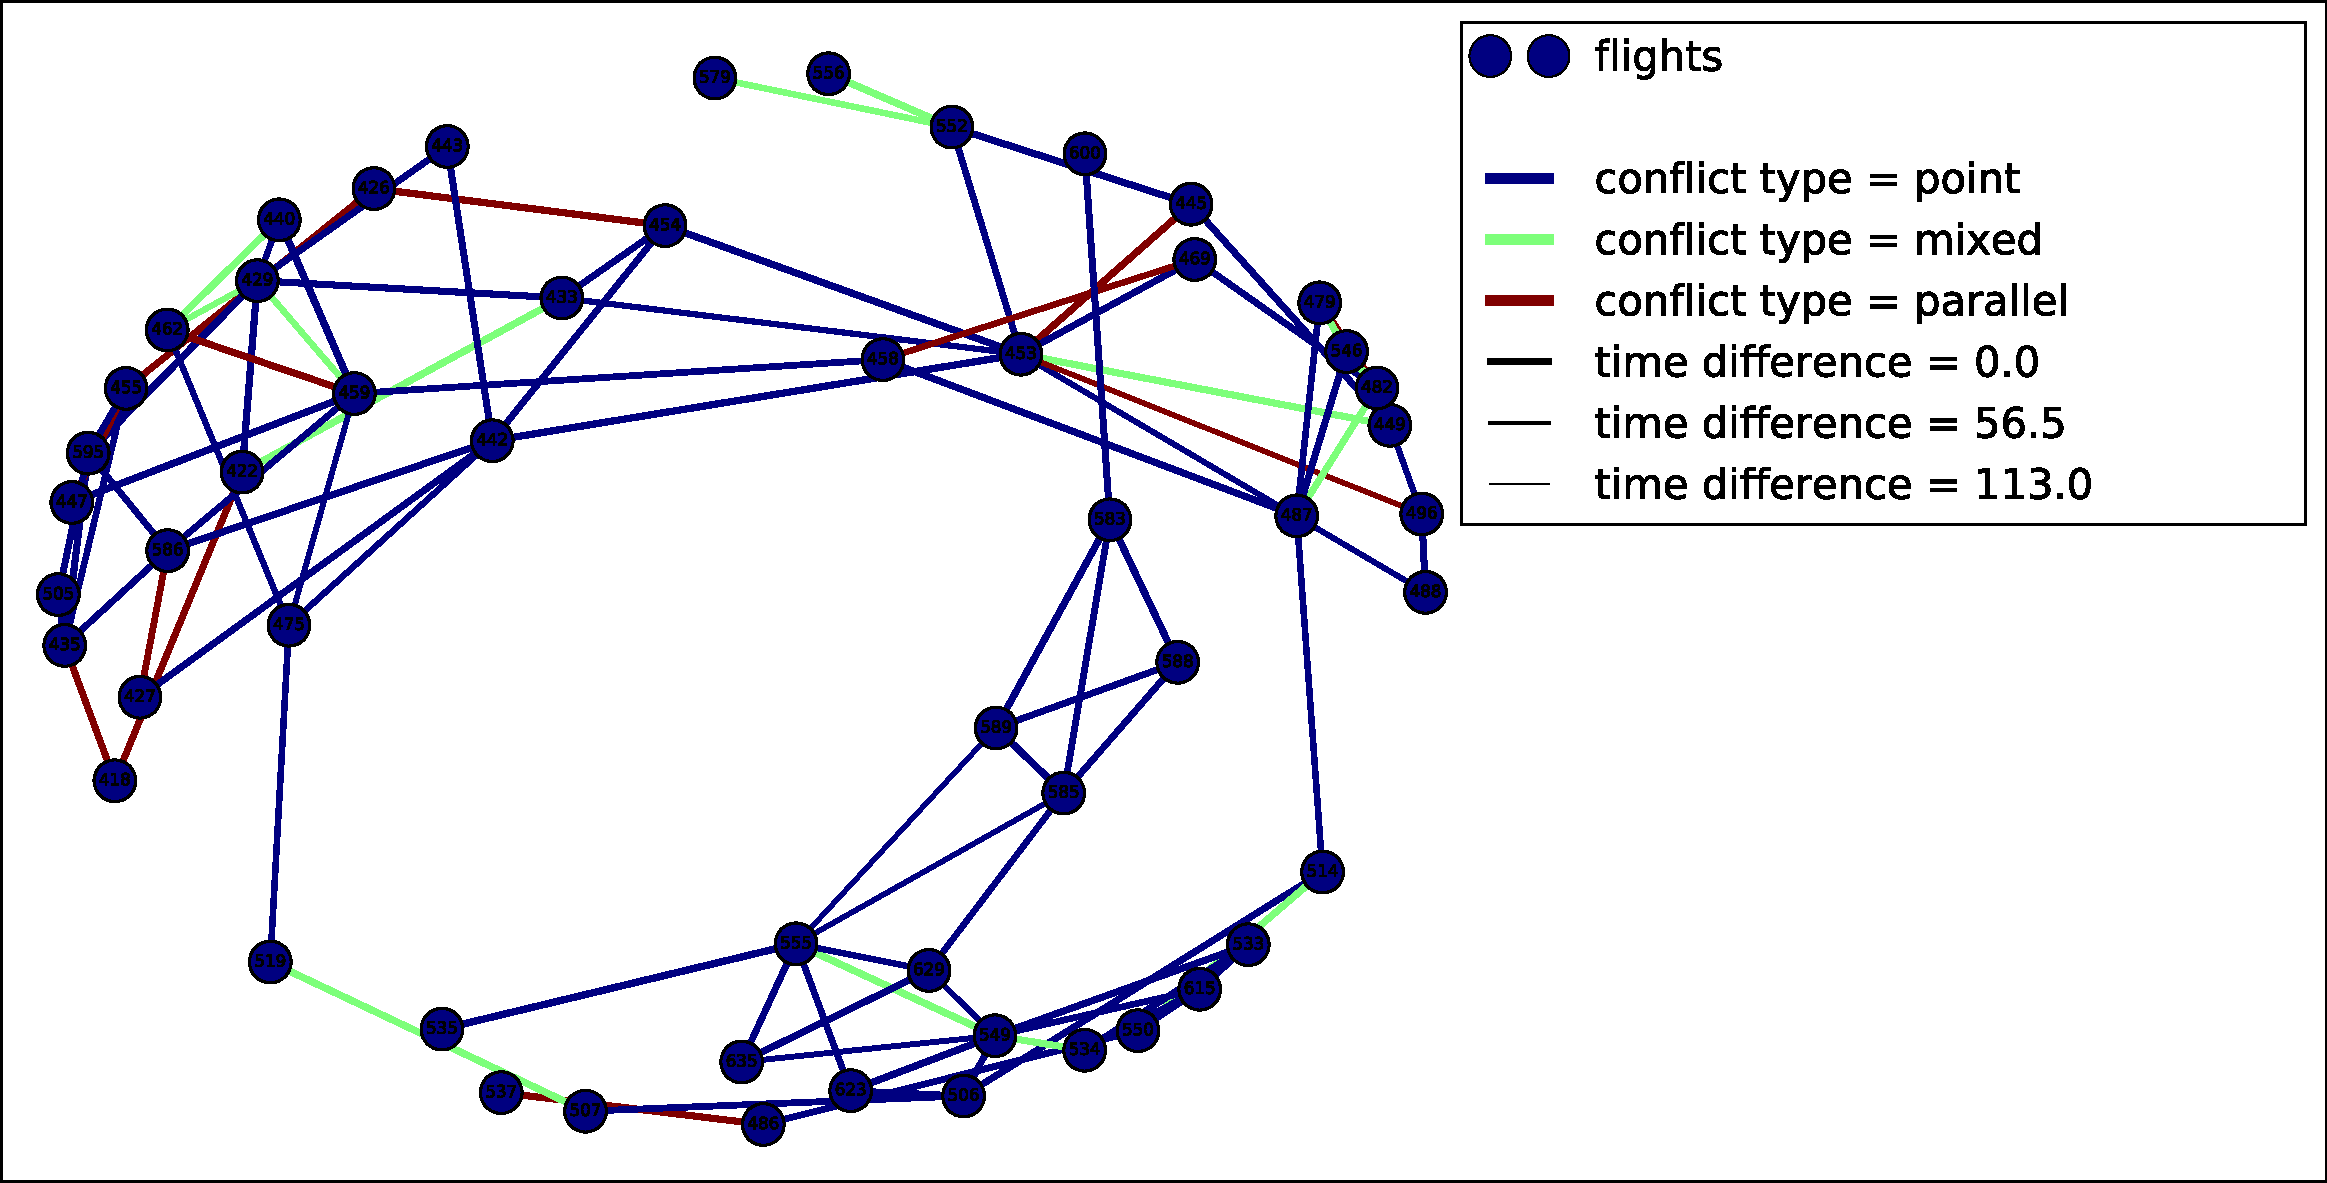
\includegraphics[width=0.85\textwidth]{images/conflicts_graph_zoom_new.pdf}
        \end{center}
    }
\end{frame}
\begin{frame}[t]{Potential Conflicts - Disconnected Subsets}
    Use disconnected subsets
    \begin{itemize}
        \item As starting point for hybrid classical-quantum approaches
        \item For solving small problems on the D-Wave quantum annealer
    \end{itemize}
\end{frame}
\begin{frame}[t]{Mapping to PUBO}
    \begin{block}{Optimization problem}
        \begin{equation*}
            \underset{d_i, d_{ik}, a_k}{\text{minimize}} \; \sum_i d_i + \sum_{ik} \mathcal{D}_{ik}(\Delta_{k}, a_k)
        \end{equation*}
        \begin{align*}
            \text{subject to} \qquad
            & \Delta_{k} = t_{ik} + d_i + \sum_{p<k} d_{ip} - t_{jk} - d_j - \sum_{q<k} d_{jq} \\
            & d_{ik} = \mathcal{D}_{ik}(\Delta_{k}, a_k) 
        \end{align*}
    \end{block}

    \begin{itemize}
        \item Restrict all variables to integers
        \item Express integers as binary variables. E.g.
            \begin{equation*}
                d_i = \sum_\alpha \alpha d_{i\alpha}\quad \text{with } d_{i\alpha} \in \{0, 1\}
            \end{equation*}
    \end{itemize}
\end{frame}
\begin{frame}[t]{Mapping to PUBO}
    \begin{block}{Polynomial Unconstrained Binary Optimization (PUBO)}
        \begin{align*}
            &\underset{d_{i\alpha}, d_{ik\beta}, \Delta_{k\delta}, a_{k\gamma}}{\text{minimize}}  \sum_{i\alpha} \alpha d_{i\alpha} 
            + \sum_{ik\beta} \beta d_{ik\beta} \\
            &+ \sum_k \left(\sum_\delta \delta \Delta_{k\delta} - t_{ik} - \sum_\alpha \alpha d_{i\alpha} - \sum_{p<k \atop \beta} \beta d_{ip\beta} + t_{jk} + \sum_\alpha \alpha d_{j\alpha} + \sum_{q<k \atop \beta} \beta d_{jq\beta}\right)^2 \\
            &+ \sum_{ik} \left(\sum_\beta \beta d_{ik\beta} - \sum_{\delta\gamma} \mathcal{D}_{ik}(\delta, \gamma)  \Delta_{k\delta} a_{k\gamma} \right)^2
            + \sum_i \left(\sum_\alpha d_{i\alpha} - 1 \right)^2 + \dots
        \end{align*}
    \end{block}
\end{frame}
\begin{frame}[t]{Mapping to PUBO}
    \begin{itemize}
        \item Binary variable for difference in arrival times
            $
            \; \Delta_{k} = \sum_\delta \delta \Delta_{k\delta}
            $
        \item Conflict avoiding term
            \vspace{-0.1cm}
            \begin{equation*}
                \sum_{ik} \left(\sum_\beta \beta d_{ik\beta} - \sum_{\delta\gamma} \mathcal{D}_{ik}(\delta, \gamma)  \Delta_{k\delta} a_{k\gamma} \right)^2
            \end{equation*}
    where
    \vspace{-0.1cm}
    \begin{equation*}
        \mathcal{D}_{ik}(\delta, \gamma) = 
        \begin{cases}
            D &\text{if } |\delta| < 3 \text{ minutes} \\
            0 &\text{else}
        \end{cases}
    \end{equation*}
    \end{itemize}
    \vspace{-0.5cm}
    \begin{center}
        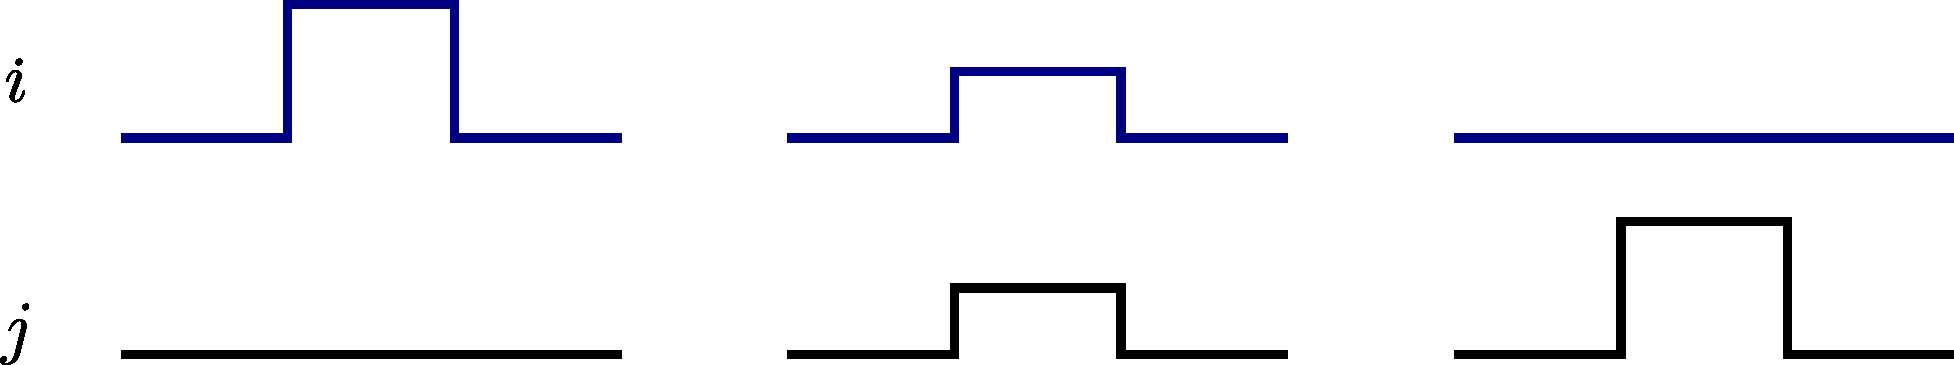
\includegraphics[width=0.76\textwidth]{images/conflict_delay_function_maneuver_without_labels.pdf}
    \end{center}
    \vspace{-0.3cm}
    \hspace{2.5cm}
    $\gamma = 0$ 
    \hspace{1.9cm}
    $\gamma=\frac{1}{2}$
    \hspace{1.9cm}
    $\gamma=1$
\end{frame}
\begin{frame}[t]{Reduction to QUBO}
   \begin{itemize}
       \item Reduce quartic and cubic terms to quadratic terms by degree reduction
       \item Drawback: More variables
   \end{itemize} 
\end{frame}
\begin{frame}[t]{Simplified Model: Only Departure Delays}
    \begin{itemize}
        \item Simplification: No maneuver delays $d_{ik}$
        \item Penalize conflicts with
            \begin{equation*}
                \mathcal{P}_k(\Delta_k) = 
                \begin{cases}
                    P & \text{ if } | \Delta_k | < 3 \text{ minutes} \\
                    0 &\text{ else }
                \end{cases}
            \end{equation*}
            where $P = $const.
    \end{itemize}
    \begin{block}{Optimization problem}
        \begin{equation*}
            \underset{d_i}{\text{minimize}} \; \sum_i d_i + \sum_{k} \mathcal{P}_k(\Delta_k)
        \end{equation*}
    \end{block}
\end{frame}
\begin{frame}[t]{Simplified Model - Mapping to QUBO}
    Difference of conflict arrival times becomes
    \vspace{-0.2cm}
    \begin{equation*}
        \Delta_k = t_{ik} - t_{jk} + d_i - d_j
    \end{equation*}
    \vspace{-0.7cm}
    \begin{block}{QUBO}
        \begin{align*}
            &\underset{d_{i\alpha}, \Delta_{k\delta}}{\text{minimize}} \; p_1 \sum_{i\alpha} \alpha d_{i\alpha} 
            + p_2 \sum_{k}\sum_{\delta \atop |\delta| < 3 \text{min}} \Delta_{k\delta} \\
            &+ p_3 \sum_k \left(\sum_\delta \delta \Delta_{k\delta} - t_{ik} - \sum_\alpha \alpha d_{i\alpha} + t_{jk} + \sum_\alpha \alpha d_{j\alpha} \right)^2 \\
            &+ p_4 \sum_i \left(\sum_\alpha d_{i\alpha} - 1 \right)^2 + p_5 \sum_k \left(\sum_\delta \Delta_{k\delta} - 1 \right)^2
        \end{align*}
    \end{block}
\end{frame}

\begin{frame}[t]{Simplified Model - Small Problem Instances}
    Generate random instances with
    \begin{itemize}
        \item Number of flights: 5, 10, 20, 50
        \item Number of random conflicts: 5, 10, 20, 50
        \item Random conflict arrival times
        \item Departure delays: $0, 3, \dots, 18$ minutes
        \item Different sets of penalty weights $p_i$
    \end{itemize}
    \begin{block}
        {Preliminary quantum annealing results from D-Wave 2X at NASA Ames (Work in progress)}
        \begin{itemize}
            \item So far, no valid solutions
            \item Possible reason: Precision issue
        \end{itemize}
    \end{block}
\end{frame}
\begin{frame}[t]{Summary and Outlook}
    \begin{block}{Summary}
        \begin{itemize}
            \item Air traffic management problems can be mapped to PUBO
            \item Significant classical preprocessing for real data
        \end{itemize}
    \end{block}
    \begin{block}{Next steps}
        \begin{itemize}
            \item Map PUBO to QUBO
            \item Investigate alternative approaches, like Jop Shop Scheduling
            \item Quantum annealing runs
        \end{itemize}
    \end{block}
\end{frame}
\end{document}

